\chapter{Countability}

\section{More on Bijections}
Recall upon the Zeroth Rule of Counting: \\
Two finite sets have the same size iff their elements can be paired up, where each element of one set has a unique partner in another. \\
This is oddly familiar. It is, in fact, formalized via the concept of bijection, which we will re-introduce here after its brief appearance when discussing modular arithmetics.
\begin{ln-define}{Bijections}{}
    Consider a function $f: A \rightarrow B$, which since it is a function, would satisfy that $\forall x \in A, f(x) \in B$. \\
    Then $f$ is a bijection if such relation holds true in a reverse direction. Therefore, for a bijection $f: A \rightarrow B$:
    \[[\forall x \in A (f(x) \in B)] \land [\forall x \in B (f(x) \in A)]\]
\end{ln-define}
In this case, as discussed before, $f$ would satisfy two other significant properties simultaneously: injective and surjective.
\begin{ln-define}{Injective, Surjective, Bijection}{}
    We call the $A$ the set of \textit{pre-images}, and $B$ the set of \textit{images}.
    \begin{bindenum}
        \item{
            \textbf{Injective}: Each image (output) has at most one pre-image (input). This type of function is thus called a "one-to-one" function.
            \begin{center}
                \begin{tikzpicture}
                    \node[circ] (A1) at (0, 0) [label=left:$A_1$] {};
                    \node[circ] (A2) at (0, 0.3) [label=left:$A_2$] {};
                    \node[circ] (B1) at (2, 0) [label=right:$B_1$] {};
                    \node[circ] (B2) at (2, 0.3) [label=right:$B_2$] {};
                    \node[circ] (B3) at (2, 0.6) [label=right:$B_3$] {};
                    \draw (A1) -- (B1);
                    \draw (A2) -- (B2);
                    \draw (0, 0.15) ellipse (0.8cm and 0.8cm);
                    \draw (2, 0.3) ellipse (0.8cm and 0.8cm);
                \end{tikzpicture}
            \end{center}
        }
        \item{
            \textbf{Surjective}: Each image (output) has at least one pre-image (input). This type of function is "onto".
            \begin{center}
                \begin{tikzpicture}
                    \node[circ] (A1) at (0, 0) [label=left:$A_1$] {};
                    \node[circ] (A2) at (0, 0.3) [label=left:$A_2$] {};
                    \node[circ] (A3) at (0, 0.6) [label=left:$A_3$] {};
                    \node[circ] (B1) at (2, 0) [label=right:$B_1$] {};
                    \node[circ] (B2) at (2, 0.3) [label=right:$B_2$] {};
                    \draw (A1) -- (B1);
                    \draw (A2) -- (B2);
                    \draw (A3) -- (B2);
                    \draw (0, 0.3) ellipse (0.8cm and 1.2cm);
                    \draw (2, 0.15) ellipse (0.8cm and 1.2cm);
                \end{tikzpicture}
            \end{center}
        }
    \end{bindenum}
\end{ln-define}
And once again, the inverse of a bijective function must also be bijective. While this is listed as an exercise to the reader, you may imagine bijections as relationship between sets $A$ and $B$; then, notice that inverse functions of $f: A \rightarrow B$ are infact relationships $f^{-1}: B \rightarrow A$. \\
Since $f^{-1}$ is the inverse of $f$, it carries the exact same pairings of $f$ and must also be bijective as $f$ is.

\subsection{Cardinality and Bijection}
Cardinality is the size of a set. \\
To show that two sets have the same cardinality, we can attempt to prove the existence of a bijection between them. \\
For example, let us consider the following problem of two sets:
\begin{ln-quest}{The cardinality of nonnegative integers and positive integers}{}
    For this course, $0 \in \N$. Essentially, we ask if the cardinality of $\N$ is equal to that of $\Z^+$. \\
    To prove the equality, let us attempt to form a bijection between these sets:
    \begin{center}
        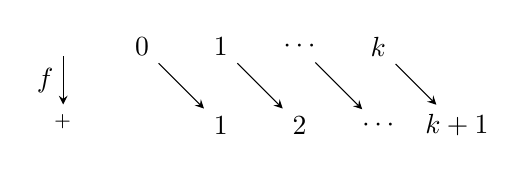
\begin{tikzpicture}
            \node (N) at (0, 1) {$\N$};
            \node (Z) at (0, 0) {$\Z^+$};
            \draw[-stealth] (N) -- (Z) node[midway, left]{$f$};
            \node (n0) at (1, 1) {0};
            \node (z1) at (2, 0) {1};
            \node (n1) at (2, 1) {1};
            \node (z2) at (3, 0) {2};
            \node (n2) at (3, 1) {$\cdots$};
            \node (z3) at (4, 0) {$\cdots$};
            \node (n3) at (4, 1) {$k$};
            \node (z4) at (5, 0) {$k + 1$};
            \draw[-stealth] (n0) -- (z1);
            \draw[-stealth] (n1) -- (z2);
            \draw[-stealth] (n2) -- (z3);
            \draw[-stealth] (n3) -- (z4);
        \end{tikzpicture}
    \end{center}
    We can see that there is indeed a bijection $f: \N \rightarrow \Z^+$, since every value of each set is paired with another value from the other set. We speak of this as: having \textbf{enumerated} each element from set $\Z^+$.\\
    Meanwhile, we can notice that the relationship is one-to-one because no two natural numbers have the same image.
\end{ln-quest}
A very similar case can be made for $f: \N \rightarrow 2\N$, and can be found on the lecture note.

We are left with another interesting case where bijection can be certified, between $\N$ and $\Z$. \\
Our initial thought here would have to do with the properties of both sets. For each pair of number $(-k, k)$ in $\Z$, where $k$ is a natural number, we also need to take two respective numbers from $\N$ to match against them. \\
If so, then let us attempt with the function:
\[
    f(x) = 
    \begin{cases}
        \frac{x}{2} &\text{if x is even} \\
        -\frac{x + 1}{2} &\text{if x is odd} \\
    \end{cases}
\]
And let us see how this pairing works out:
\begin{center}
    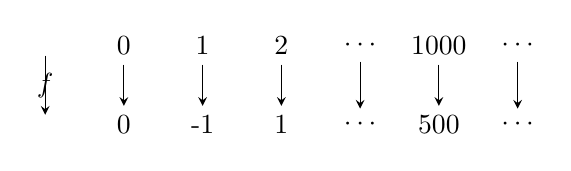
\begin{tikzpicture}
        \node (N) at (-1, 1) {$\N$};
        \node (Z) at (-1, 0) {$\Z$};
        \node (n0) at (0, 1) {0};
        \node (n1) at (1, 1) {1};
        \node (n2) at (2, 1) {2};
        \node (n3) at (3, 1) {$\cdots$};
        \node (n4) at (4, 1) {1000};
        \node (n5) at (5, 1) {$\cdots$};
        \node (z0) at (0, 0) {0};
        \node (z1) at (1, 0) {-1};
        \node (z2) at (2, 0) {1};
        \node (z3) at (3, 0) {$\cdots$};
        \node (z4) at (4, 0) {500};
        \node (z5) at (5, 0) {$\cdots$};
        \draw[-stealth] (N) -- (Z) node[midway]{$f$};
        \draw[-stealth] (n0) -- (z0);
        \draw[-stealth] (n1) -- (z1);
        \draw[-stealth] (n2) -- (z2);
        \draw[-stealth] (n3) -- (z3);
        \draw[-stealth] (n4) -- (z4);
        \draw[-stealth] (n5) -- (z5);
    \end{tikzpicture}
\end{center}
Let us proceed with a proof of its bijection by demonstrating its injectiveness and surjectiveness:
\begin{ln-quest}{Prove the One-to-One and Onto of above function}{}
    Remember that to prove a realtionship $f$ as bijection, we will be proving its two substatements:
    \begin{bindenum}
        \item \textbf{Injectiveness}: $\forall x, y \in \U, f(x) = f(y) \implies x = y$
        \item \textbf{Surjectiveness}: $\forall y, \exists x, f(x) = y$
    \end{bindenum}

    \textbf{Injectiveness (One-to-One)}: \\
    Suppose there exists two arbitrary values $x, y$ such that $f(x) = f(y)$. \\
    Then, both values must have the same sign, so either $f(x) = \frac{x}{2} = f(y) = \frac{y}{2}$ or $f(x) = -\frac{x + 1}{2} = f(y) = -\frac{y + 1}{2}$. \\
    And in either case, we obtain that $x = y$, thus obtaining that:
    \[f(x) = f(y) \implies x = y\]
    Therefore, $f$ is injective.
    
    \textbf{Surjectiveness (Onto)}: \\
    Suppose that $y$ is non-negative, then $f(2y) = y$. Suppose that $y$ is negative, then $f(-(2y + 1)) = y$ as well. \\
    Since every image has a pre-image, $f$ is onto.
\end{ln-quest}

Therefore, while $\N$ has the same size with $\Z^+$, it also has the same size with $\Z$. Interesting!

\section{Countability}
Now we come to an imporatant question. What does it mean for a set to be countable? 
\begin{ln-define}{Countability}{}
    A set $S$ is countable if it is finite, or if there is a bijection between $S$ and $N \subseteq \N$.
\end{ln-define}
Essentially, if we can enumerate all members of a set $S$, then the set $S$ is countable. Vice versa.

Well, just knowing countability by definition would yield fun, but what would yield more fun? Explaining if $|\Q| = |\N|$!
\begin{ln-think}{Proof that $|\N| = |\Q|$}{}
    To do so, let us first observe that $|\N| \leq |\Q|$, since we would see that every natural number is a rational number while the reverse does not necessarily hold true. \\
    
    To continue off this proof, we now need to recognize if also $|\Q| \leq |\N|$. \\
    To do so, we will exhibit an injection $f: \Q \rightarrow \N$.
    
    Now, let us consider a counterclockwise spiral that rotates its direction of travel 90 degrees counterclockwise. In such a figure, findable from the lecture notes (Around page 4), we observe that each rational number is represented by the point (x, y) on the path of such spiral, which is placed on the two-dimensional space $\Z^2$.
    
    If we map each lattice point on the spiral to the numeric order of its precedence on the spiral, we then thus prove that every rational number (characterized as a lattice point, again) must correspond to one natural number. \\
    Therefore, knowing that all points on the spiral must be presentable as a natural number, and knowing that each lattice point corresponds to exactly one natural number: $|\Q| \leq |\N|$.

    Last but not least:
    \[
        |\N| \leq |\Q| \land |\Q| \leq |\N| \implies |N| = |Q|
    \]
\end{ln-think}

\begin{ln-think}{Proof that the set of all polynomials is countable}{}
    The set of all binary strings is countable: each binary strings has a representative number, and if we must consider the empty string, then we would assign it to the value $0$ and assign other bit-strings to the number they represent in binary base added by $1$. \\
    This exact reasoning would suffice for ternary strings, quad-ary strings, hexadecimal strings... the list goes on, but this holds a significant implication.
    \begin{quote}
        If we can manage to map mathematical objects, like polynomials and graphs (representable by adjacency matrices, for example), then sets of matheamtical objects can indeed also be proven as countable.
    \end{quote}
    The lecture note proposes an example proving the set of all polynomials to be countable, via formatting a polynomial as a ternary string, where each coefficients and exponents are formatted in their binary bit-string form and separated by a character ``2''.
    The former logic has stated that the set of all ternary strings is countable, which would then, via convenience offered from the definition of countability, make the set of all polynomials be as countable as the set of all ternary strings are.
\end{ln-think}

Now, on a similar note, let's prove a much more significant proposition in scale:
\begin{ln-think}{Proof that the Cartiesian product of countable sets is countable}{}
    Let countable sets $S$ and $T$ be examined for the proof, where we prove that $S \times T$ is countable. \\
    We should first observe that $S$ and $T$ themselves must, for their countability, have injections:
    \begin{align*}
        f: S \rightarrow \N \\
        g: T \rightarrow \N
    \end{align*}
    Therefore, there must also exist some injection:
    \[h: S \times T \rightarrow \N \times \N\]
    where $S \times T$ is a set of tuples of enumerated items, so representable as a set of tuples of natural numbers.

    Then, let us investigate the countability of $\N^2$. \\
    We recognize that each natural number larger than $1$ has a unique prime factorization. Therefore, let us enumerate all ordered pairs $(x, y) \in \N^2$ with the number $2^x 3^y$ (2 and 3 here are replaceable by other prime numbers). \\
    Then, we will have built an injection with the above rules:
    \begin{align*}
        F: \N^2 \rightarrow \N \\
        F(x, y) := 2^x 3^y
    \end{align*}
    where the relation $F$ is indeed injective because each number can only have one unique prime factorization, such that:
    \[
        \forall m, n, r, s \in \N, (2^m 3^n = 2^r 3^s \implies m = r \land n = s)
    \]
    Now, such injection suggests that $\N^2$ is countable; therefore, $S \times T$, which has an injection towards $\N^2$, must also be countable.
\end{ln-think}

\section{Cantor's Diagonalization}
In this chapter, we deal with two great questions. \\
First of all, rational numbers are so dense? The set of rational numbers is dense, as between any two rational numbers, we can find another rational number. In fact, between any two real numbers there is always a rational number (which we used as an example in Chapter 2 when demonstrating proofs). It's Real Dense.

And second of all, is there a bijection between the rationals and the reals, provided the above fact of the density of set (that real numbers and rational numbers are all dense)? We will resolve this question via an argument from Cantor, known as ``Cantor\'s diagonalization''.

But, before presenting the proof, let us recall that any real number in the interval $[0, 1]$ can be written as an infinite decimal with no trailing zeros, and rational numbers can be represented as recurring decimals, while irrational ones non-recurring decimals. \\
Most importantly, all decimal expressions of irrational numbers are all unique and infinitely long. For numbers like $0.5$, they will be represented as $0.4\overline{9}$.
\begin{ln-theorem}{Uncountability of Real Numbers}{}
    \textbf{Theorem}: The real interval $\R[0, 1]$ is uncountable.
    \tcblower
    \textbf{Proof}: For the sake of contradiction, let us consider there is a bijection $f: \N \rightarrow \R[0, 1]$. We may then enumerate real numbers in an infinite list $f(0), \cdots$ as follows:
    \begin{align*}
        f(0) &= 0.5214\cdots \\
        f(1) &= 0.1416\cdots \\
        f(2) &= 0.9478\cdots \\
        f(3) &= 0.5309\cdots \\
        \vdots &\vdots \vdots
    \end{align*}
    The basic rule of this construction is that for the number of leftup-rightdown diagonal (in this case $0.5479\cdots$) $r$, its ${(i + 1)}^{th}$ digit after decimal point must be same with that of $f(i)$ for any $i \in \N$. \\
    However, we can see that a value, such as $r$ whose digit is incremented by $2$ under modulo $10$, cannot fit into this enumeration because of its ${(i + 1)}^{th}$ digit not being equal to that corresponding digit of $r$. \\
    Therefore, we see at least one item not counted in the ``bijection'' that should've existed between $\N$ and $\R[0, 1]$, thus deeming $\R[0, 1]$ uncountable.
\end{ln-theorem}
The way this technique worked ultimately roots in how we defined a real number as an infinite decimal expansion that can be either recurring or non-recurring. Say today we attempt to apply this argument on $\Q$, which is a set of recurring decimal expansions, the proof wouldn't gain progress because we cannot confirm whether the number of diagonal is indeed a recurring decimal representation. \\
In other words, Cantor's Diagonalization relies on the infinite length of expressions from the set it attempts to prove uncountable.

\section{Cantor's Set}
The Cantor's Set then argues about the mathematical properties of interval $\R[0, 1]$. This set is defined by repeatedly removing the middle thirds of line segments infinitely many times.
\begin{ln-define}{Cantor's Set, Defined by Construction}{}
    A Cantor's Set can be constructed iteratively with infinite steps. \\
    In each step, we remove the middle one-third of line segments we currently have. For example,
    \[[0, 1] \rightarrow \bigg[ 0, \frac{1}{3} \bigg] \cup \bigg[ \frac{2}{3}, 1 \bigg]\]
    And then we proceed to remove the middle third of each line segments we deal with:
    \[\bigg[0, \frac{1}{3} \bigg] \cup \bigg[\frac{2}{3}, 1 \bigg] \rightarrow \bigg[0, \frac{1}{9} \bigg] \cup \bigg[\frac{2}{9}, \frac{1}{3} \bigg] \cup \bigg[\frac{2}{3}, \frac{7}{9} \bigg] \cup \bigg[\frac{8}{9}, 1 \bigg]\]
\end{ln-define}
You would think that the Cantor's Set faces an inevitable emptiness (just like most of human life), but it is merely that the measure of the set is zero, as in it now contains many almost trivial intervals with many isolated points across the interval and ``looks mathematically like being empty''. It is the realistic equivalent of looking at a white paper with many atomic black points, which we just cannot perceive with human eyes. \\
But the Cantor's Set is uncountable. This is proven by forming a bijection between the Cantor's Set and an uncountable set:
\begin{ln-theorem}{The Uncoutnability of Cantor's Set}{}
    \textbf{Theorem}: The Cantor's Set is uncountable.
    \tcblower
    \textbf{Proof}: Each element in the Cantor's Set can in fact be expressed as a ternary string, at last containing only those whose ternary representations have $0$s and $2$s (because those that involve $1$s must have been in the middle third of some interval and thus deserves removal). \\
    We will also proceed to write any finite decimal expressions into its infintie form (for example, $0.1 \rightarrow 0.0\overline{2}$). \\
    This leaves us with a set builder representation of the Cantor's Set:
    \[
        \bigg\{C = \{x \in [0, 1]: \text{x has a ternary representation of only 0s and 2s}\} \bigg\}
    \]
    Which allows us to map the set $C$ onto the interval $\R[0, 1]$ via substituting every trit $2$ with value $1$ and forcing the ternary string into a binary presentation that corresponds to some value in $\R[0, 1]$. \\
    This way, we formed a bijection between $C$ and an uncountable set, so using the Zeroth Rule of Counting, $C$ the Cantor's Set is also uncountable.
\end{ln-theorem}
Note that the difference between the above proof and the proof of countability for sets of all binary string, is that in the Cantor's Set proof, leading $0$-valued bits exist, as supposed to them not existing in the enumerable set of bitstrings.

\section{Power Sets: Higher Order Infinity}
Here is a review on Power Sets:
\begin{ln-define}{Power Set}{}
    The power set of $S$ can be written as:
    \[\mathbb{P} (S) = \{P | P \subseteq S\}\]
    as one of its various denotations, the one on lecture note using a Weierstrass P, $\wp$. \\
    The power set of a set is the set of all of its possible subsets.
\end{ln-define}
In addition, if the cardinality of $S$ in the above definition is $|S| = k$, then we can state that $|\mathbb{P} (S)| = 2^k$. \\
This can now be combinatorically understood: every power set is a $k$-bit string representation for the absence of each of $k$ elements. \\
Now, let us discuss if the power set of $\N$ can be countable, and from there, reveal a thing or two about infinity.
\begin{ln-theorem}{Uncountability of $\wp(\N)$}{}
    For the sake of contradiction, let us assume there is a bijection $f: \N \rightarrow \wp (\N)$ defined exactly like Cantor's Diagonalization Argument, where each row of a table describes a subset via a bit-string, and each column stands for whether an element of $\N$ is present or not. \\
    Let us now present a modified version of the diagonal number (again, leftup-rightdown) that is the flipped version of diagonal (which means $0$s and $1$s are flipped). That digit then must not exist in the enumeration, therefore proving the bijection malfunctional, and moreover,
    \[|\wp(\N)| > |\N|\]
\end{ln-theorem}
The cardinality of $\N$ is denoted in the symbol $\aleph_0$ (aleph-null), and using that symbol, $|\wp(\N)| = 2^{\aleph_0}$. \\
Such cardinality of $\wp(\N)$ is the same as the cardinality of $\R$, which is known as \textbf{c}. \\
Even larger infinite cardinalities are denoted as $\aleph_k$ where $k > 0$, and they can be defined using set theory. They, interestingly, obey the rules of arithmetics, and in turn provide assistance towards famous mathematical hypotheses.
